\documentclass{article}
\usepackage{afterpage}
\usepackage{float}
\usepackage{longtable}
\usepackage{graphicx}
\usepackage{pdflscape}
\usepackage[numbers,sort&compress]{natbib}
\usepackage{psfrag}

\usepackage{amsmath}
\usepackage{amsfonts}
\usepackage{graphicx}
\usepackage{nicefrac}
\usepackage{graphicx}
\usepackage{caption}
% \usepackage{subcaption}
\usepackage{subfigure}
% \usepackage{algorithm}
% \usepackage{paralist}
% % \usepackage[geometry]{ifsym}
\usepackage{rotating}
%
\newcommand{\uu}[1]{\boldsymbol #1}
\usepackage{listings}
\usepackage{xcolor}
\lstset{language=C++,
                keywordstyle=\color{blue},
                stringstyle=\color{red},
                commentstyle=\color{green},
                morecomment=[l][\color{magenta}]{\#}
}
\begin{document}

\section*{MHD - Neumann bilinear form}

The variational for the MHD model with inhomogeneous Neumann conditions is
\begin{equation}
\label{eq:VariationForm}
\begin{split}
A(\uu{u}_h,\uu{v}) + O(\uu{u}_h;\uu{u}_h,\uu{v}) +C(\uu{b}_h;\uu{v},\uu{b}_h) +B(\uu{v}, p_h) & =  (\uu{f},\uu{v})_\Omega - (\uu{p_N},v)_{\Omega_N}\\
B(\uu{u}_h,q)&= 0, \\
M(\uu{b}_h,\uu{c})-C(\uu{b}_h;\uu{u}_h,\uu{c})+ D(\uu{c},r_h)&= (\uu{g},\uu{c})_\Omega,\\
D(\uu{b}_h,s)&=0,
\end{split}
\end{equation}
where $\uu{p_N}$ is the Neumann condition. Then the Picard iteration is given by:
\begin{equation}
\label{eq:picard}
\begin{split}
A(\delta\uu{u}_h, \uu{v}) +O({\uu{u}_h};\delta\uu{u}_h,\uu{v})+ C(\uu{b}_h;\uu{v},\delta \uu{u}_h) + B(\uu{v}, \delta p_h) & = R_u(\uu{u}_h,\uu{b}_h,p_h;\uu{v}),\\
B(\delta\uu{u}_h,q)&= R_p(\uu{u}_h;q),\\
M(\delta \uu{b}_h,\uu{c})+
D(\uu{c},\delta r_h)-C(\uu{b}_h;\delta \uu{u}_h,\uu{v})&= R_b(\uu{u}_h,\uu{b}_h,r_h;\uu{c}),\\
D(\delta \uu{b}_h,s)&= R_r(\uu{b}_h;s),
\end{split}
\end{equation}
where
\begin{equation}
\label{eq:RHSpicard}
\begin{split}
 R_u(\uu{u}_h,\uu{b}_h,p_h;\uu{v})=&(\uu{f}, \uu{v})_\Omega- (\uu{p_N},v)_{\Omega_N}-A(\uu{u}_h,\uu{v})
-  O(\uu{u}_h;\uu{u}_h,\uu{v})\\
& - C(\uu{b}_h;\uu{v},\uu{b}_h)-B(\uu{v},p_h),\\
R_p(\uu{u}_h;q)=&-B(\uu{u}_h,q),\\
 R_b(\uu{u}_h,\uu{b}_h,r_h;\uu{c})=&(\uu{g,c})_\Omega -M(\uu{b}_h,\uu{c})
+ C(\uu{b}_h;\uu{u}_h,\uu{c})-D(\uu{c},r_h),\\
R_r(\uu{b}_h;s)=&-D(\uu{b}_h,s),
\end{split}
\end{equation}
Therefore you need to enforce the inhomogeneous Neumann conditions at each non-linear iteration???? Also, if you enforce homogeneous boundary conditions within the non-linear iteration doesn't this stop model from capturing the pressure driven flow?

\section*{MHD - smooth Neumann conditions}

Consider the exact solution:
\begin{figure}[h!]
    \centering
    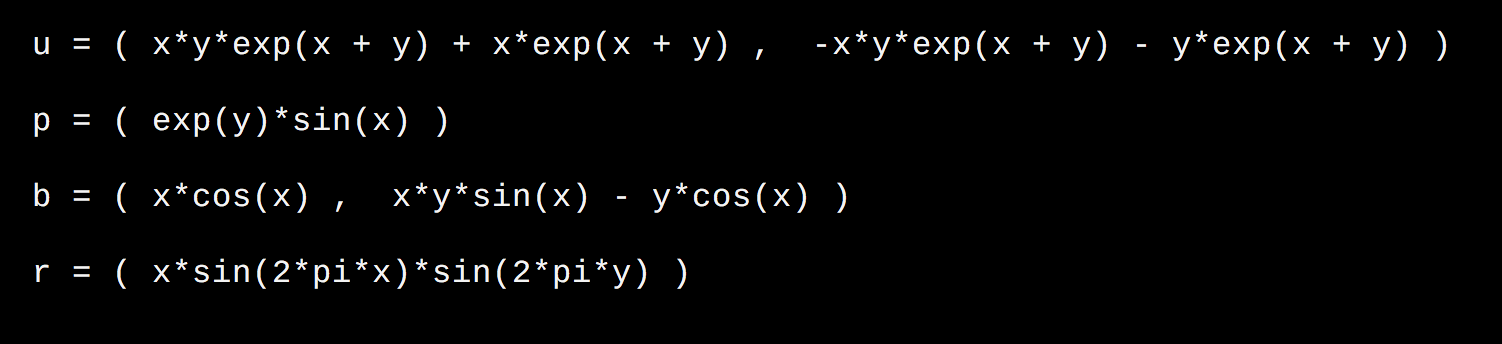
\includegraphics[width=\textwidth]{Solution}
\end{figure}


The error tables are given below. Here I used a unit square domain with Neumann conditions on the left and right boundaries and Dirichlet on the top and bottom ones.
\begin{table}[h!]
\begin{center}
\begin{tabular}{cccccccc}
\hline \hline

$\ell$ &    Dofs $\uu{u}_h/p_h$ & $\|\uu{e}_u\|_{L^2(\Omega)}$ & $r$ & $\|\uu{e}_u\|_{H^1(\Omega)}$ & $r$ &$\|e_p\|_{L^2(\Omega)}$ & $r$  \\
\hline
\hline
1 &      50/9 &  9.0942e-02 &     - &  1.2457e+00 &     - &  5.6315e-01 &      - \\
2 &     162/25 &  1.1441e-02 &     3.53 &  3.2338e-01 &     2.29 &  7.8755e-02 &      3.85 \\
3 &     578/81 &  1.3656e-03 &     3.34 &  8.1946e-02 &     2.16 &  9.2087e-03 &      3.65 \\
4 &    2,178/289 &  1.6719e-04 &     3.17 &  2.0637e-02 &     2.08 &  1.0929e-03 &      3.35 \\
5 &    8,450/1,089 &  2.0858e-05 &     3.07 &  5.1826e-03 &     2.04 &  1.6142e-04 &      2.88 \\
6 &   33,282/4,225 &  2.6265e-06 &     3.02 &  1.2990e-03 &     2.02 &  3.1921e-05 &      2.39 \\
7 &  132,098/16,641 &  2.7450e-07 &     3.28 &  3.2522e-04 &     2.01 &  7.4632e-06 &      2.12 \\
\hline\hline
\end{tabular}

\caption{Convergence for 2D MHD - fluid variables}
\label{tab:MHD_2D_smooth_fluids_velocity}
\end{center}
\end{table}


\begin{table}[h!]
\begin{center}
\begin{tabular}{cccccccccc}
\hline
\hline
$\ell$ &    Dofs $\uu{b}_h/r_h$ & $\|\uu{e}_b\|_{L^2(\Omega)}$ & $l$ & $\|\uu{e}_b\|_{H({\rm curl},\Omega)}$ & $l$ \\
\hline\hline
 1 &     16/9 &  1.8060e-01 &     - &  2.6788e-01 &        - \\
 2 &     56/25 &  9.1265e-02 &     1.09 &  1.3398e-01 &        1.11 \\
 3 &    208/81 &  4.5753e-02 &     1.05 &  6.7003e-02 &        1.06 \\
 4 &    800/289 &  2.2892e-02 &     1.03 &  3.3503e-02 &        1.03 \\
 5 &   3,136/1,089 &  1.1448e-02 &     1.01 &  1.6752e-02 &        1.01 \\
 6 &  12,416/4,225 &  5.7241e-03 &     1.01 &  8.3759e-03 &        1.01 \\
 7 &  49,408/16,641 &  2.8621e-03 &     1.00 &  4.1879e-03 &        1.00 \\
\hline\hline

\end{tabular}
\caption{Convergence for 2D MHD  - magnetic variable}
\label{tab:MHD_2D_smooth_magnetic}
\end{center}
\end{table}



\begin{table}[h!]
\begin{center}
\begin{tabular}{cccccccccc}
\hline
\hline
$\ell$ &    Dofs $\uu{b}_h/r_h$ & $\|\uu{e}_r\|_{L^2(\Omega)}$ & $l$ & $\|\uu{e}_r\|_{H^1(\Omega)}$ & $l$ \\
\hline\hline
  1 &     16/9 &  2.7524e-01 &     - &  2.4780e+00 &     - \\
  2 &     56/25 &  1.4850e-01 &     1.21 &  1.7787e+00 &     0.65 \\
  3 &    208/81 &  4.8879e-02 &     1.89 &  1.0042e+00 &     0.97 \\
  4 &    800/289 &  1.3198e-02 &     2.06 &  5.1942e-01 &     1.04 \\
  5 &   3,136/1,089 &  3.3659e-03 &     2.06 &  2.6198e-01 &     1.03 \\
  6 &  12,416/4,225 &  8.4572e-04 &     2.04 &  1.3128e-01 &     1.02 \\
  7 &  49,408/16,641 &  2.1170e-04 &     2.02 &  6.5676e-02 &     1.01 \\
\hline\hline

\end{tabular}
\caption{Convergence for 2D MHD  - multiplier variable}
\label{tab:MHD_2D_smooth_multiplier}
\end{center}
\end{table}


\section*{MHD - Hartmann Neumann conditions}

\subsection*{Small domain - $(0,10)\times(1,1)$}


\subsection*{Large domain - $(0,50)\times(1,1)$}



\end{document}

